\chapter{Data processing}
\label{ch:data_processing}

The events recorded by the \hisparc electronics consist of the \pmt readouts (traces) and the trigger timestamp. Before the events can be used in analysis observables have to be extracted from the traces. For the reconstructions the particle count and arrival time for each detector are used. These values can be derived from the traces and trigger timestamp. The following sections will detail each step of the processing.

\section{Online processing}
\label{sec:online}

% On the HiSPARC PC
% This data is sent to/stored in the datastore (Table 3.1 Fokkema);
% ext_timestamp, data_reduction, trigger_pattern, baseline, std_dev, n_peaks, pulseheights, integrals, traces, event_rate
When the \hisparc electronics trigger the detected signal traces and timing information is sent to the controlling PC. First the PC determines the absolute \gps timestamp for the event. The PC then analyses each trace individually to determine several event properties.


\subsection{Trace baseline}

Though the \adcs are calibrated the baselines can still shift away from the desired value. Therefore the baseline must be determined for each trace. There is a high probability that the pre-trigger window part of the event traces do not contain a significant signal. If there was a large signal if would likely have been part of the trigger. Moreover, the rate of singles is low enough that the probability of a coincidental signal is less than \SI{0.1}{\percent}. Hence the first part of traces is suitable for determining their baselines. An algorithm checks if the signal is smooth enough by calculating a cumulative moving average and comparing each sample to the average and previous sample \cite{oostenbrugge2014daq}. At least the first 50 samples must satisfy the smoothness criteria. If that is the case then the average of those samples will be the baseline. If the start of the trace is not smooth the baseline can not be determined and will be set to the error value \num{-999}. The algorithm has recently been updated to also attempt to find a baseline from the end of the trace if it does not succeed from the start, this is not retroactively applied. Once the baseline is known other properties can be determined, if the baseline can not be determined all other properties are also set to \num{-999}. The baseline determination will fail if the first part of the trace contains a peak. Also signal oscillations (caused by a bad \pmt) can cause the baseline determination to fail. However, in the case of large oscillations the trigger may have been caused by the oscillations, so the data is bad.


\subsection{Signal strength}

The pulse height is the value of the highest signal in the trace, relative to the baseline. With the baseline calibrated to \SI{200}{\adc} the highest possible pulse height is $4096 - 200 = \SI{3896}{\adc}$. For most stations this value is rarely attained, because most \pmts are unable to produce large enough signals. For stations with new \pmts saturated signals occur multiple times per day. For each triggered event in a 2-detector station, using the default triggering, both detectors should have a pulse height at least equal to the low threshold, since that is the trigger condition. This may fluctuate due to fluctuations in the baseline, since the trigger thresholds are not relative to the actual baseline. For events triggered in 4-detector stations there are often two detectors with very small or no significant pulses. Most events are triggered by two high signals in two detectors, with no signals in the other two detectors.  

The pulse integral is the sum of the signals that are at least \SI{20}{\adc} above the baseline. This threshold filters signal noise, reflections, and small peaks. In \cref{fig:integral} these two observables are illustrated.

\begin{figure}
    \centering
    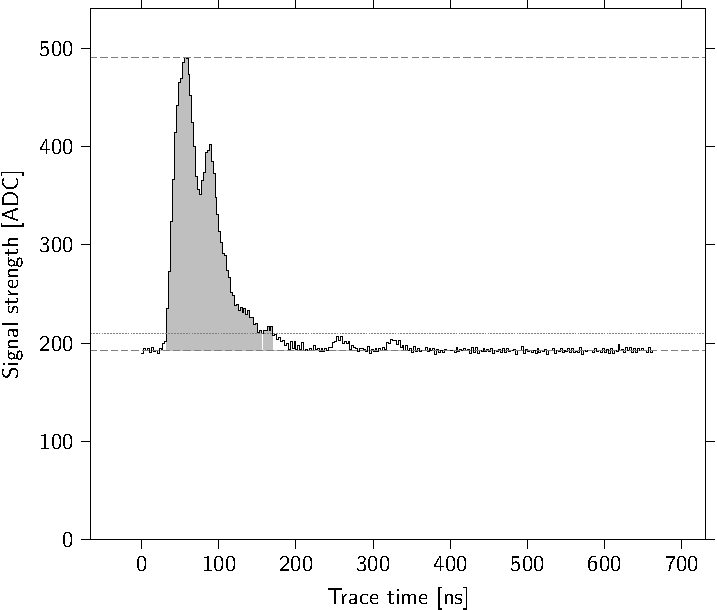
\includegraphics[width=0.7\linewidth]{plots/processing/integral}
    \caption{Illustrated definition of the pulse height and integral for a signal trace (solid line). The baseline (lower dashed line) was determined using the pre-trigger window of the trace (not shown). The pulse height is the space between the two dashed lines. The integral is indicated by the shaded area, only signals above the threshold (dotted line) count towards the integral.}
    \label{fig:integral}
\end{figure}


\subsection{Signal structure}

Most traces contain only a single pulse. However, sometimes multiple particle pass through a detected within the short time window of the trigger, and separated enough to be distinguishable in the trace. In order to find events with multiple pulses the number of peaks in a trace is determined. This starts at the start of a trace and when the signal values rise more than the low threshold (relative to the baseline) a peak is counted. When a peak has reached its apex and then lowers again the maximum value is remembered, the value needs to drop at least the value of the threshold before a new peak can start. For the next peak the signal value needs to rise at least the threshold value again, above the new local minimum. The number of peaks is also a good indication of light leaks, which result in many small peaks in traces. The ratio between the pulse height and integral also provides structure information. If the pulse integral is higher than expected (see pmt linearity test or ph v integral plot) for a given pulse height then the trace probably contains multiple peaks.

[illustrate with figure]

As a measure of the stability of the trace around the baseline the standard deviation of the same part of the trace that was used for the baseline is calculated. This can be an indicator for the misalignment of the \adcs.

At each event the average trigger rate (\si{\hertz}) as measured by the \daq over the last 90 seconds is added to the event. The first few events when starting the \daq will have a to low trigger rate due to the lack of information from the 90 seconds preceding the first trigger. Though not a property of the event itself, this provides insight in the proper operation of the detection station.


\subsection{Data reduction}

Most events contain only two pulses in two detectors. These pulses are often very correlated in time (at least within the \SI{1.5}{\micro\second} trigger window) and normal small pulses are \SIrange{30}{100}{\ns} long. The rest of the trace is usually empty, and contains no valuable data. For each event the part containing all significant pulses is determined. The algorithm looks from the start and end of the traces up to the point that any of the detectors has a pulse. The empty parts of the traces will be cut away, some padding is added to allow verification of the baseline in the offline analysis. On average (median) this leads to traces with \SI{150}{\ns} (i.e. 60 samples) length. The default trace length (pre-trigger, trigger, post-trigger windows) is \SI{6}{\micro\second} (i.e. 2400 samples). Overall \SI{2.5}{\percent} of the measured data is kept. This greatly reduces the size of data to be transferred to the datastore and to be analysed offline. In order to have more baseline information every \SI{40}{\minute} the full traces of an event are kept. This allows for a quality check of the baselines.

[figure with part of (more than reduced) full trace showing the cutoffs]

% Scipt to determine some values, to be determined for larger dataset:
% lengths = [zlib.decompress(s.blobs[i]).count(',') for i in range(0, s.blobs.nrows, 4)]
% median(lengths)
% mean([l for l in lengths if l != 2400])
% len([l for l in lengths if l ==2400])


\subsection{Mean/Noise filter}

During the setup of a station the separate \adcs for each channel in the \hisparc electronics are aligned, however, this alignment is not perfect and can change over time. Typically a saw-tooth pattern can be observed in the measured traces. The amplitude of the saw-tooth can be different at different signal levels, because both the offset and gain may be different. This can be filtered out by averaging the signal. This is a multi-step process. First the trace is split into the even and odd parts (positive and negative clock) which are smoothed separately. These smoothed signals are interleaved and then smoothed again. The smoothing algorithm can be configured to prevent smoothing of signals significantly different from surrounding signals, in order to preserve real pulses. 

This is a destructive method in which information is lost. For the \hisparc stations at the Science Park the filtering has been disabled, to preserve raw trace values. The negative effect of trace filtering is described in \cref{sec:trigger_time}. The most recent version of the \hisparc \daq implements this filter only for the display on the \hisparc PC. The data will be sent to the datastore unfiltered. If desired the filter can be applied in the offline analysis.

\begin{figure}
    \centering
    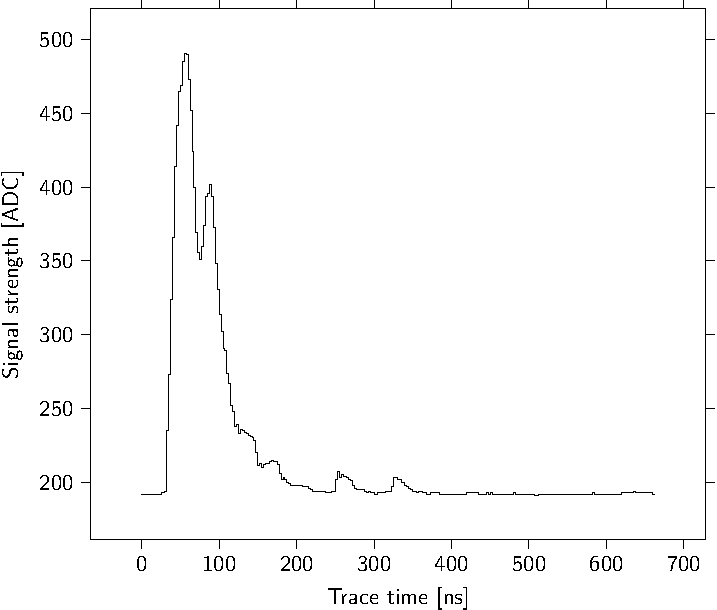
\includegraphics[width=0.7\linewidth]{plots/processing/mean_filter}
    \caption{The same trace as shown in \cref{fig:integral}, except this one is filtered using the Mean Filter. The small peaks and baseline are noticeably smoother.}
    \label{fig:mean_filter}
\end{figure}


\subsection{Trigger pattern}

The \hisparc events contain a trigger pattern which indicates which trigger thresholds (including the external trigger) were active during the trigger window, which of the comparators were triggered, and the presence of a slave. A threshold being set to `on' in the trigger threshold pattern does not mean that that threshold actively contributed to the trigger. Take for example a 4-detector station which triggers on 2 high signals. If 2 simultaneous high signals in channels 1 and 2 cause a trigger, then several nano seconds later (still in the trigger window) a high signal appears in channel 3, the high threshold for channel 3 will be marked as active, even though that channel did not actively contribute to the trigger. Therefore it is better to look at the traces to determine what caused the trigger. Moreover, due to a software bug the trigger pattern was stored incorrectly for most data, missing part of the pattern. The trigger pattern is not used in the further analysis.


\subsection{Event data from PC}

The events contain ... when sent from the PC.


\section{Offline processing for the Event Summary Data}

Every morning, several hours after midnight, all new data is processed to generate the Event Summary Data (ESD). Several hours after midnight is used because some stations may be slow in uploading data, this allows extra time to let all events from the previous day come in.  The event processing also looks for older dates with new events, not just yesterday. Stations have a local buffer in case they are temporarily unable to upload data. There have been cases where a station had several months worth of data locally which was all uploaded once the connection was reestablished. By keeping track of modification dates to the raw data files (stored by date) it is easy to find dates with new data. The processing applies the event processing module from \sapphire to the data. The following section describe exactly what this involves.

The first step is the sorting of the events by timestamp, since events are not always uploaded in the correct order. Next duplicate events are removed. Duplicate events can occur when uploading a batch of events takes to long and \python has a timeout, while Windows continues to upload in the background. The \python program will try to upload the data again because it believes the upload failed.


\subsection{Number of particles}

The size of the signals is a measure for the number of particles which passed though the detector. The pulse integral will be used for this since it also accounts for particles which arrive separately in time. Moreover, as shown in \cref{sub:pmt_linearity} the integral is less hindered by saturation of the \adcs. In order to relate the pulse integral to a number of particles the signal strength for a single particle needs to be determined. This is done separately for each detector, since each may be calibrated differently. To determine the signal for a single particle pulse integral data from multiple events is required. As shown in \cref{fig:ph_histogram_contrib} the pulse height histogram is a combination of contributions by a different number of particles and gamma's, the same is true for the pulse integral. By taking a day's worth of events the peak, which is Most Probable Value (\mpv) for a single particle, becomes apparent. By fitting this value a good estimate for the signal of a single particle is achieved.

[figure of pulse integral histogram with fitted MPV]


\subsection{Trigger time}
\label{sec:trigger_time}

For each event a \gps timestamp is recorded at the moment the trigger conditions are met. Unfortunately, no data is included which connects the \gps timestamp to a specific sample of the traces. This is needed to relate traces from different events and stations. In order to find the sample in the traces to which the \gps timestamp belongs the trigger has to be reconstructed from the trace. Since the trigger conditions are known this simply requires applying the trigger logic to the traces. For each channel look if and when it crosses the low and high thresholds. Then find which trigger conditions are met, and which are first. For a 2-detector station this is simply the second channel that crosses the low threshold. For a 4-detector station either the second high or third low signal, which ever is first. However, the \hisparc electronics trigger on the raw traces which the \adcs read out, but if the Mean Filter is active in the \daq the traces are filtered before they are transmitted to the datastore. The filter sometimes smoothes trace such that signals that actually crossed a threshold no longer do so in the filtered trace. In some cases this makes it impossible to reconstruct the trigger. However, this is only the case where low signals or slow rising signals were part of the trigger.

\begin{figure}
    \centering
    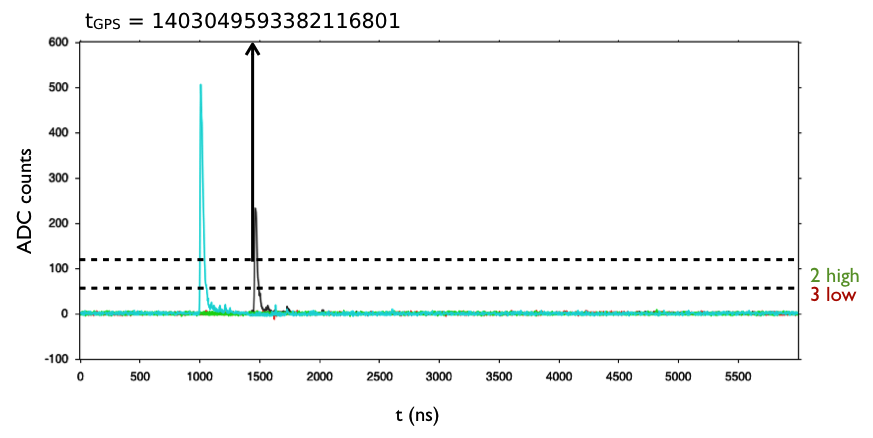
\includegraphics[width=0.7\linewidth]{plots/processing/trigger_time.png}
    \caption{The reconstruction of the trigger time within a trace. For this 4-detector station event the trigger was caused by 2 high signals.}
    \label{fig:trigger_time}
\end{figure}


\subsection{Arrival times}

The arrival time of particles in each individual detector is used for direction  reconstruction. The arrival time is defined at the start of the first pulse in a detector, as illustrated in \cref{fig:arrival_time}. Using the \gps timestamp and trigger time these arrival times can be converted to \gps time using $t_{i,\gps} = t_\gps - t_{trigger} + t_i$.

\begin{figure}
    \centering
    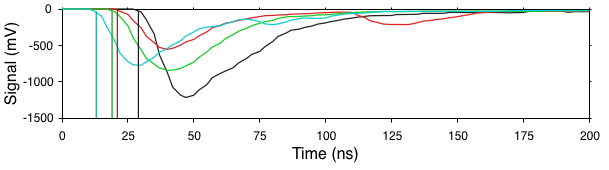
\includegraphics[width=0.7\linewidth]{plots/processing/arrival_time.png}
    \caption{The reconstruction of the arrival time within traces.}
    \label{fig:arrival_time}
\end{figure}


\subsection{Detector offsets}

Time offsets are observed between detectors as reported in \cref{sec:detector-offsets}. These need to be corrected for correct direction reconstruction. One day of data is enough to determine these offsets for the detectors within a station.

All events that triggered a combination of two detectors. Calculate at all arrival time differences. Ideally the mean would be \SI{0}{\ns}, standard deviation related to the distance between the detectors. However, there is often an offset of several nano seconds. Distribution of offsets.. see section station.


\subsection{Coincidences}

Finally all processed events from all stations of a day are sorted into a long list. Then coincidences between stations are found. A coincidence is a group of least two events for which the \gps timestamps are within \SI{10000}{\ns}. All unique combinations of events which are not subsets of other combinations are stored.


\subsection{Station offsets}

Finally the offset between stations is determined. More than a single day of data is required for this. As reported in [ref station offsets section]. The amount of time required to determine an accurate station offsets depends on the number of coincidences between the stations, from ... follows the coincidence rate between stations as a function of their distance. However, as shown in [ref width distance] the width of the time difference distribution increases with distance between the stations, as an effect of inclined showers and shower front curvature. With enough coincidences these effects average out and a good offset can bet determined. When the distance between stations is very large the expected \gps offsets of up to \SI{100}{\ns} [check value] become less important as they have less effect on the direction reconstruction. At a distance of .. meters a difference of 100 ns only changes the direction by ... (from Zenith)...

In some cases pairs of station are separated by a large distance but have stations between them that are closer to both. For instance stations 505 and 509 are separated by ... 600 meters, yet between them is station 501, separated 300 meter from both. There are far more coincidences between 501-505 and 501-509 than 505-509. Using 501 as a stepping stone reduces the time window required to determine an offset between 505-509, and in


\section{Data analysis}

\subsection{Shower front arrival time}

\subsection{Particle density}


\section{Data quality}

\subsection{Day}

\subsection{Events}

\subsubsection{Implementation problems}

As mentioned in the \cref{sec:online} there were some bugs in the software which caused the malformed trigger pattern, traces cut to small, and destructively filtered traces. These were fixed in the \hisparc station software version released at the end of 2015. Most stations still operate on the old version of the software. The cause is that the for some events the trigger time reconstruction fails, which prevents the event from being used in coincidence direction reconstruction. On a daily basis this results in \SI{0.2 \pm 0.1}{\percent} failed trigger time reconstructions. In these events the maximum signal strength will be just above the trigger threshold, and reduced just below it by the filter.


\subsection{Detector}
